\documentclass[tikz]{standalone}
\begin{document}
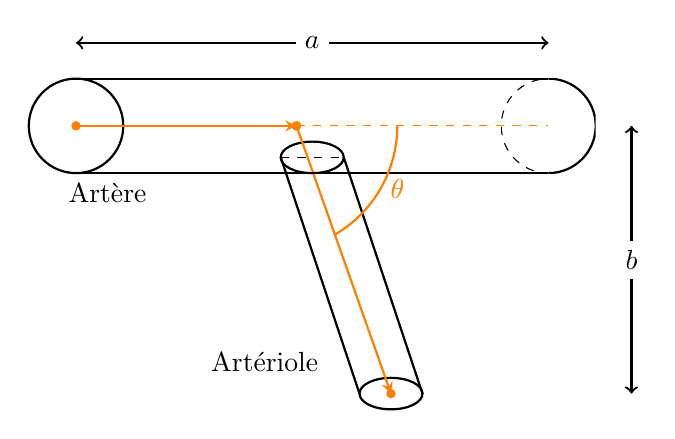
\begin{tikzpicture}[scale=2]
    % Dessine l'artère
   \begin{scope}
    \clip (3,0.3) rectangle (3.3,-0.3);
    \draw[thick] (3,0) circle (0.3);
   \end{scope}
   \begin{scope}
    \clip (2.7,0.3) rectangle (3,-0.3);
    \draw[dashed] (3,0) circle (0.3);
   \end{scope}

   \draw[thick] (0,0) circle (0.3);
    \draw[thick] (0,0.3) -- (3,0.3);
    \draw[thick] (0,-0.3) -- (3,-0.3);


    % Dessine l'artériole
    \draw[thick] (1.5,-0.2) ellipse (0.2 and 0.1);
    \draw[dashed] (1.3,-0.2) -- (1.7,-0.2);
    \draw[thick] (2,-1.7) ellipse (0.2 and 0.1);
    \draw[thick] (1.3,-0.2) -- (1.8,-1.7);
    \draw[thick] (1.7,-0.2) -- (2.2,-1.7);
    
    % Dessine les flèches
    \draw[->,>=stealth,orange,thick] (0,0) -- (1.4,0);
    \draw[thick,fill=orange,draw=none] (0,0) circle (0.03);
    \draw[thick,fill=orange,draw=none] (1.4,0) circle (0.03);
    \draw[dashed,orange] (1.4,0) -- (3,0);
    \draw[->,>=stealth,orange,thick] (1.4,0) -- (2,-1.7);
    \draw[thick,fill=orange,draw=none] (1.4,0) circle (0.03);
    \draw[thick,fill=orange,draw=none] (2,-1.7) circle (0.03);

    \draw[thick] (0,-0.3) -- (3,-0.3);
    \node[below] at (0.2,-0.3) {Artère}; 
    \node[left] at (1.6,-1.5) {Artériole};
    \draw[thick,orange] (2.04,0) arc (0:-60:0.8) node[midway,right] {$\theta$}; % Angle theta placé a 40°

    \draw[<->,thick,yshift=15] (0,0) -- (3,0) node[midway,fill=white] {$a$};
    \draw[<->,thick,xshift=15] (3,0) -- (3,-1.7) node[midway,fill=white] {$b$};

\end{tikzpicture}
\end{document}